% Topic #1 - Introduction

%------------------------------------
% Main Settings
%------------------------------------
\documentclass[10pt]{beamer}

%--------------------------------------%
% Set font, and frame title info    %
%--------------------------------------%
\usefonttheme{serif}
\setbeamerfont{frametitle}{series=\bfseries}
\setbeamerfont{framesubtitle}{series=\bfseries}

%--------------------------------------
% "Sub-settings"
%--------------------------------------
\setbeamertemplate{navigation symbols}{}		% Get rid of navigation symbols
\setbeamertemplate{items}[default]				% Uses triangles and numbers instead of 3D balls (which I don't like)
\setbeamertemplate{itemize items}[circle]		% Use circles instead of triangles for itemized lists

%-------------------------------------
% Custom Commands
%-------------------------------------
\newtheorem{hypothesis}{Hypothesis}

%---For Footnotes---%
\usepackage{tikz}
\usetikzlibrary{positioning,calc} % Needed to make angle connector arrows.
\usepackage[absolute,overlay]{textpos}
\newenvironment{reference}[2]{%
	\begin{textblock*}{\textwidth}(#1,#2)
		\tiny\bgroup\color{gray}}{\egroup\end{textblock*}}
%------%		

%----------------------------------------%
% For making definitions in boxes        %
%----------------------------------------%
\usepackage{tcolorbox}

%-- Packages for making nice tables --%
\usepackage{booktabs}
\usepackage{makecell}  % Required for specifying multiple rows within a table cell

%--------------------------------%
%     Custom Colours             %
%--------------------------------%
\usepackage{xcolor}
\definecolor{myblue}{rgb}{0,0.3,0.6}
\definecolor{myblue2}{rgb}{0,0.4,0.8}
\setbeamercolor{frametitle}{fg=myblue}
\setbeamercolor{framesubtitle}{fg=myblue2}
\setbeamercolor{itemize item}{fg=myblue}
\setbeamercolor{itemize subitem}{fg=myblue2}
\setbeamercolor{enumerate item}{fg=myblue}
\setbeamercolor{enumerate subitem}{fg=myblue2}


%----------------------------------%
% Creating nice blocks             %
%----------------------------------%
\setbeamercolor{block title}{bg=myblue, fg=white} %bg=background, fg=foreground
\setbeamercolor{block body}{bg=myblue!20, fg=black} %bg=background, fg=foreground
\setbeamerfont*{block title}{family=\sffamily, series=\bfseries, size=\large}
\setbeamertemplate{blocks}[rounded][shadow=true]

%------------------------------------------
%  Begin Presentations
%------------------------------------------
\begin{document}


%-----------------------%
%  Title Slide          %
%-----------------------%
\begin{frame}
	\begin{tikzpicture}[remember picture,overlay]
		\fill[color=myblue, draw=none] (current page.west) rectangle(current page.north east);
		\node at (2.7, 1.0) {\color{white}\LARGE{\textbf{FRSC/BIOL 4002:}}};
		\node at (2.5, 0.2) {\color{white}\LARGE{\textbf{Wildlife Forensics}}};
		\node at (0.82, -1.2) {\color{black}\normalsize{Tim Frasier}};
		\node at (1.8, -1.65) {\color{black}{\emph{Saint Mary's University}}};
	\end{tikzpicture}
\end{frame}


%------------------------%
%    Introductions       %
%------------------------%
\begin{frame}[t]
\frametitle{Introductions}
\vspace{0.5cm}
	
	\begin{center}
		\textbf{Dr. Tim Frasier}
	\end{center}
	
	\vspace{0.25cm}
	
	\begin{columns}
		\begin{column}{0.33\textwidth}
			\begin{center}
				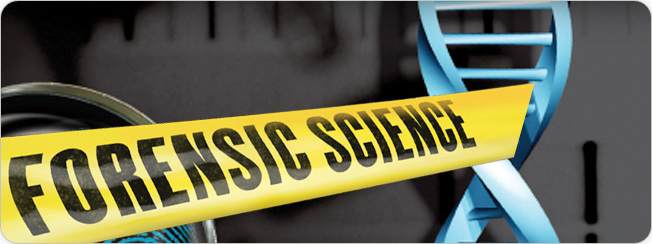
\includegraphics[width=1.0\textwidth]{figures/forensics.jpg}
			\end{center}
		\end{column}
		
		\begin{column}{0.33\textwidth}
			\begin{center}
				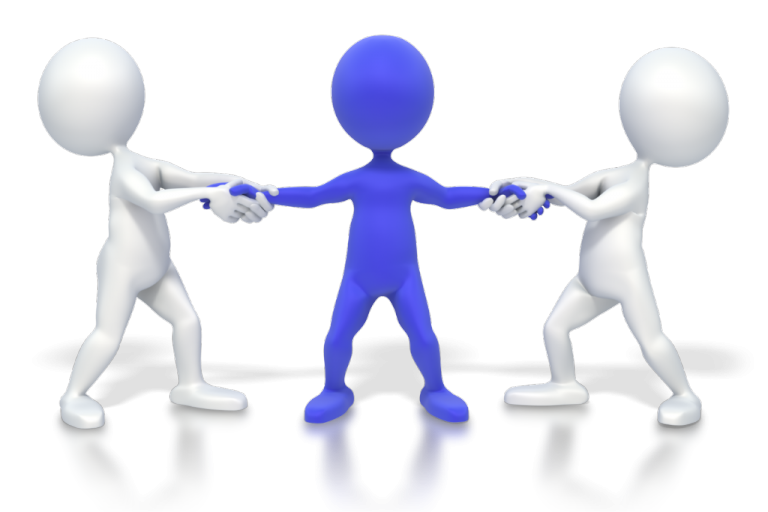
\includegraphics[width=1.0\textwidth]{figures/pulled.png}
			\end{center}
		\end{column}
		
		\begin{column}{0.33\textwidth}
			\begin{center}
				
\includegraphics[width=1.0\textwidth]{figures/biology2.jpg}
			\end{center}
		\end{column}
	\end{columns}
\end{frame}


%--------------------------%
%    Research              %
%--------------------------%
\begin{frame}[t]
\frametitle{Research}

	\begin{center}
		Conservation genetics of endangered whale species
	\end{center}

	\begin{columns}[t]
		\begin{column}{0.5\textwidth}
			\begin{center}
				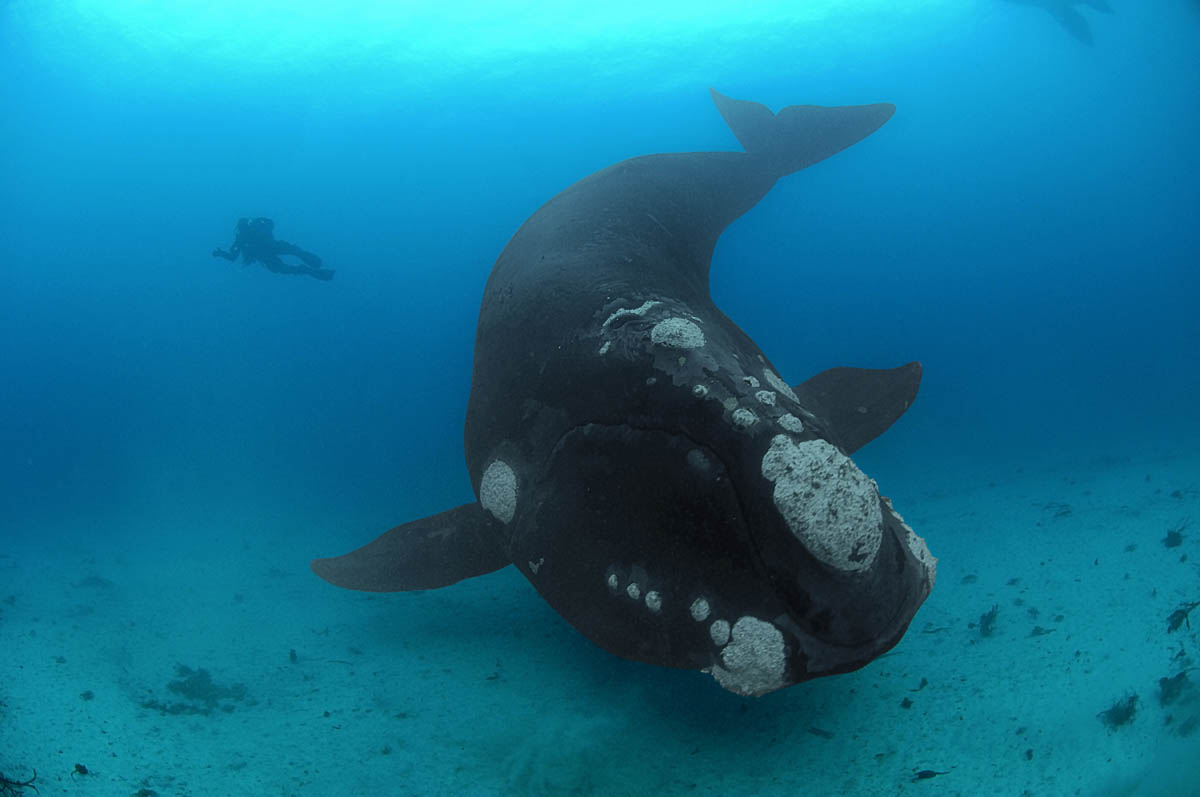
\includegraphics[width=0.8\textwidth]{figures/rightwhale.jpg}\\
				\vspace{0.25cm}
				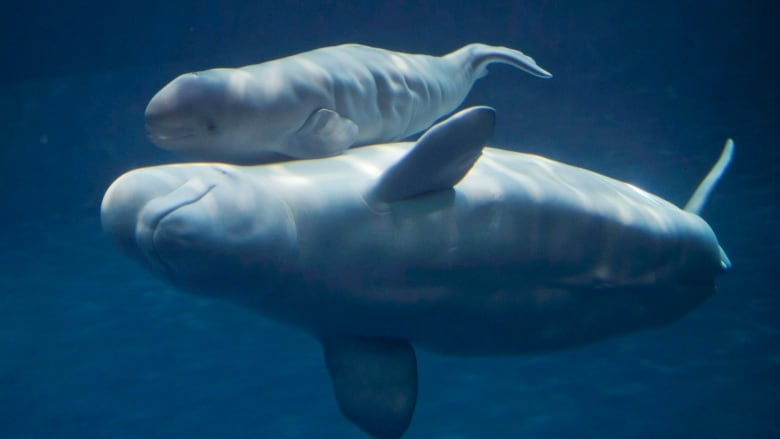
\includegraphics[width=0.8\textwidth]{figures/beluga.jpg}
			\end{center}
		\end{column}
		
		\begin{column}{0.5\textwidth}
			\begin{center}
				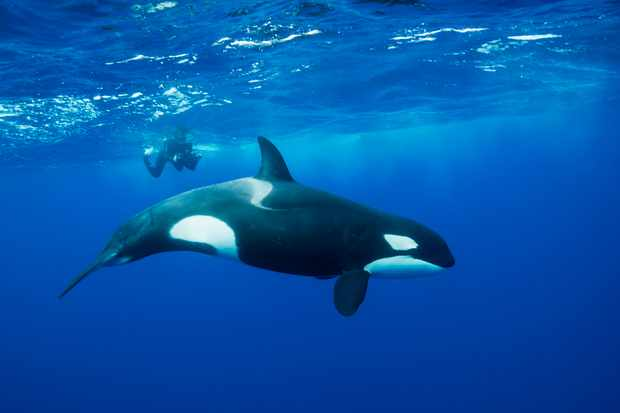
\includegraphics[width=0.7\textwidth]{figures/orca.jpg}\\
				\vspace{0.25cm}
				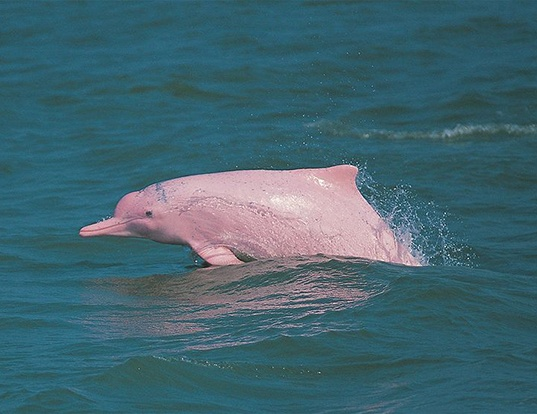
\includegraphics[width=0.7\textwidth]{figures/humpback.jpg}
			\end{center}
		\end{column}	
	\end{columns}	
\end{frame}


%---------------------------%
%   Forensics               %
%---------------------------%
\begin{frame}[t]
\frametitle{Forensics}
\vspace{0.25cm}

	\begin{center}
		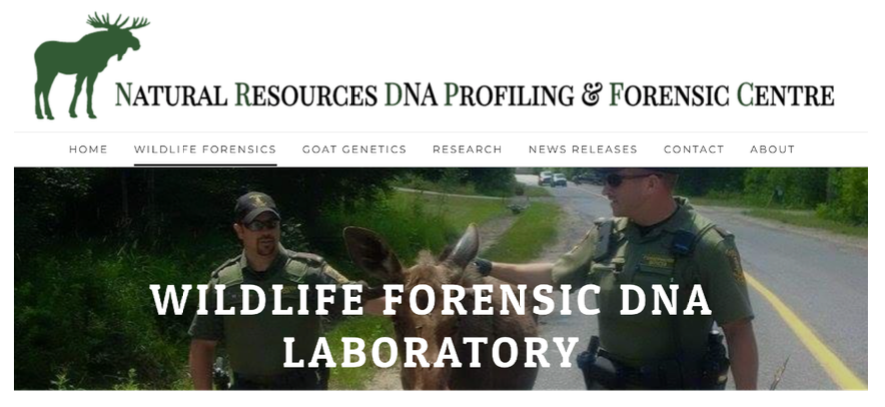
\includegraphics[width=0.6\textwidth]{figures/nrdpfc.png}\\
		\vspace{0.5cm}
		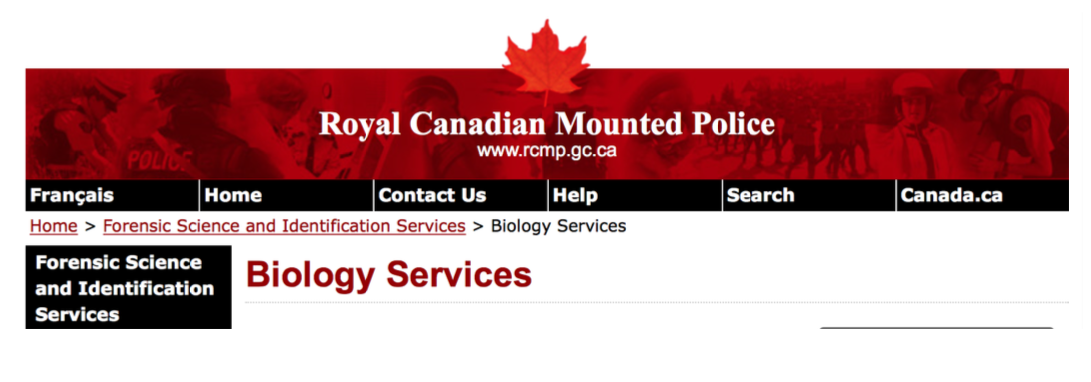
\includegraphics[width=0.6\textwidth]{figures/rcmp.png}
	\end{center}
\end{frame}


%-----------------------%
%  Cycling              %
%-----------------------%
\begin{frame}
	\begin{columns}
		\begin{column}{0.6\textwidth}
			\begin{center}
				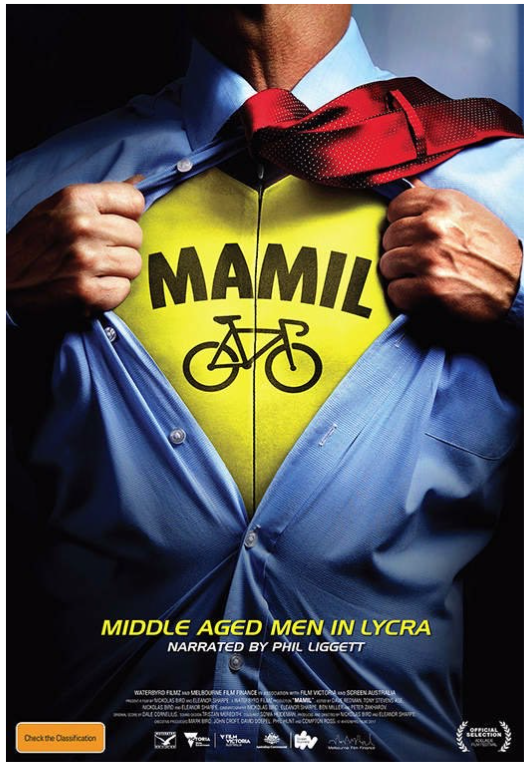
\includegraphics[width=0.75\textwidth]{figures/mamil.png}
			\end{center}
		\end{column}
		
		\begin{column}{0.4\textwidth}
			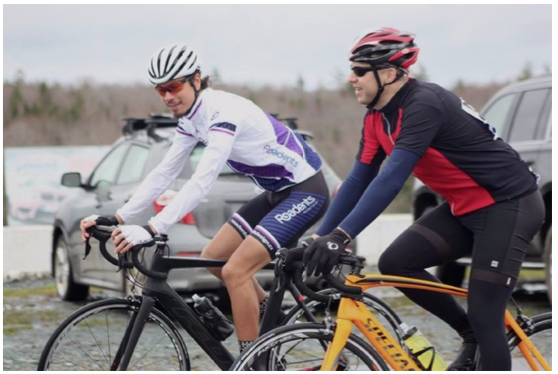
\includegraphics[width=0.9\textwidth]{figures/cycling1.png}\\
			\vspace{0.5cm}
			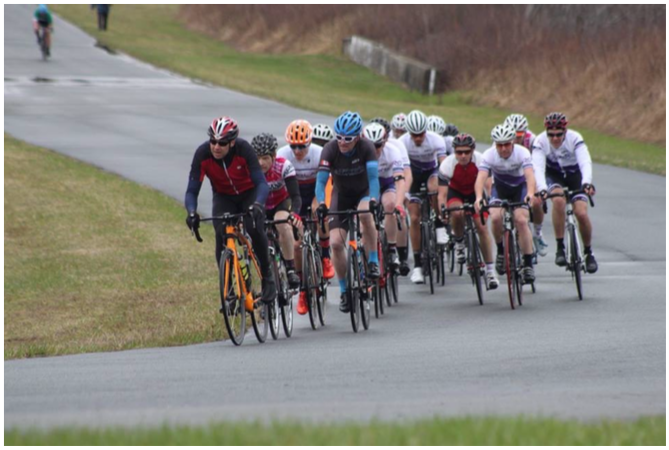
\includegraphics[width=0.9\textwidth]{figures/cycling2.png}\\
		\end{column}
	\end{columns}
\end{frame}


%-----------------------%
%  Contact Information  %
%-----------------------%
\begin{frame}[t]
\frametitle{Contact Information}
\vspace{0.5cm}

	\begin{tabular}{@{} l l}
		\textbf{Office:} & Science Building, room S 327\\
		\addlinespace
		\addlinespace
		\textbf{Tel:} & 902-491-6382\\
		\addlinespace
		\addlinespace
		\textbf{E-mail:} & timothy.frasier@smu.ca\\
				& \textcolor{myblue2}{\emph{Please put FRSC/BIOL 4002 in subject line}}\\
		\addlinespace
		\addlinespace
		\textbf{Office Hours:} & TR 1:00--4:00 \textcolor{myblue2}{\emph{or via E-mail!}}\\
	\end{tabular}
\end{frame}


%-----------------------%
%  Students             %
%-----------------------%
\begin{frame}[t]
\frametitle{Your Turn}
\vspace{0.5cm}
	
	\begin{itemize}
		\item Name?
		\medskip
		\item Are you a BIOL or FRSC (or both) student?
		\medskip
		\item What year are you in?
		\medskip
		\item Why did you take this course?
		\medskip
		\item What do you hope to get out of it?
	\end{itemize}
\end{frame}


%-----------------------%
%  Course Information   %
%-----------------------%
\begin{frame}[t]
\frametitle{Course Information}
\vspace{0.5cm}

	\begin{tabular}{@{} l l l l}
		\textbf{Lectures:} & MW & 1:00--2:15 & S345\\
		\addlinespace
		\textbf{Labs:} & W & 2:30--5:29 & S106\\
	\end{tabular}

	\vspace{1.0cm}

	\textbf{Textbook:} None, but required readings will be posted online.
	
	\vspace{1.0cm}
	
	Course material will be available on \textbf{Brightspace}
		\begin{itemize}
			\item Syllabus
			\item Readings
			\item Lecture notes
			\item etc.
		\end{itemize}
\end{frame}


%-----------------------%
%  Grades               %
%-----------------------%
\begin{frame}[t]
\frametitle{Grades}
\vspace{0.5cm}

	\begin{center}
		\begin{tabular}{@{} l r}
			\toprule
			\textbf{Component} & \textbf{\% of Final Grade}\\
			\addlinespace
			\midrule
			Case study presentation \& discussion & 20\%\\
			\addlinespace
			Lab books (2 @ 12.5\% each) & 25\%\\
			\addlinespace
			Midterm Exam & 25\%\\
			\addlinespace
			Final Exam & 30\%\\
			\midrule
			\textbf{Total} & \textbf{100\%}\\
			\bottomrule
		\end{tabular}
	\end{center}
\end{frame}


%-----------------------%
%  Lectures             %
%-----------------------%
\begin{frame}[t]
\frametitle{Lectures}
\vspace{0.5cm}

	Goals are to understand:
	
		\begin{enumerate}
			\item Major drivers of wildlife forensic issues, nationally \& internationally
			\item Major species/organisms involved
			\item The legal parties, laws, and regulations involved
			\item The conservation, environmental, and ethical issues involved
		\end{enumerate}
\end{frame}


%-----------------------%
%  Approach             %
%-----------------------%
\begin{frame}[t]
\frametitle{Approach}
\vspace{0.5cm}

 Combine lectures with case studies\\
 
 \vspace{0.5cm}
 
 	\begin{center}
		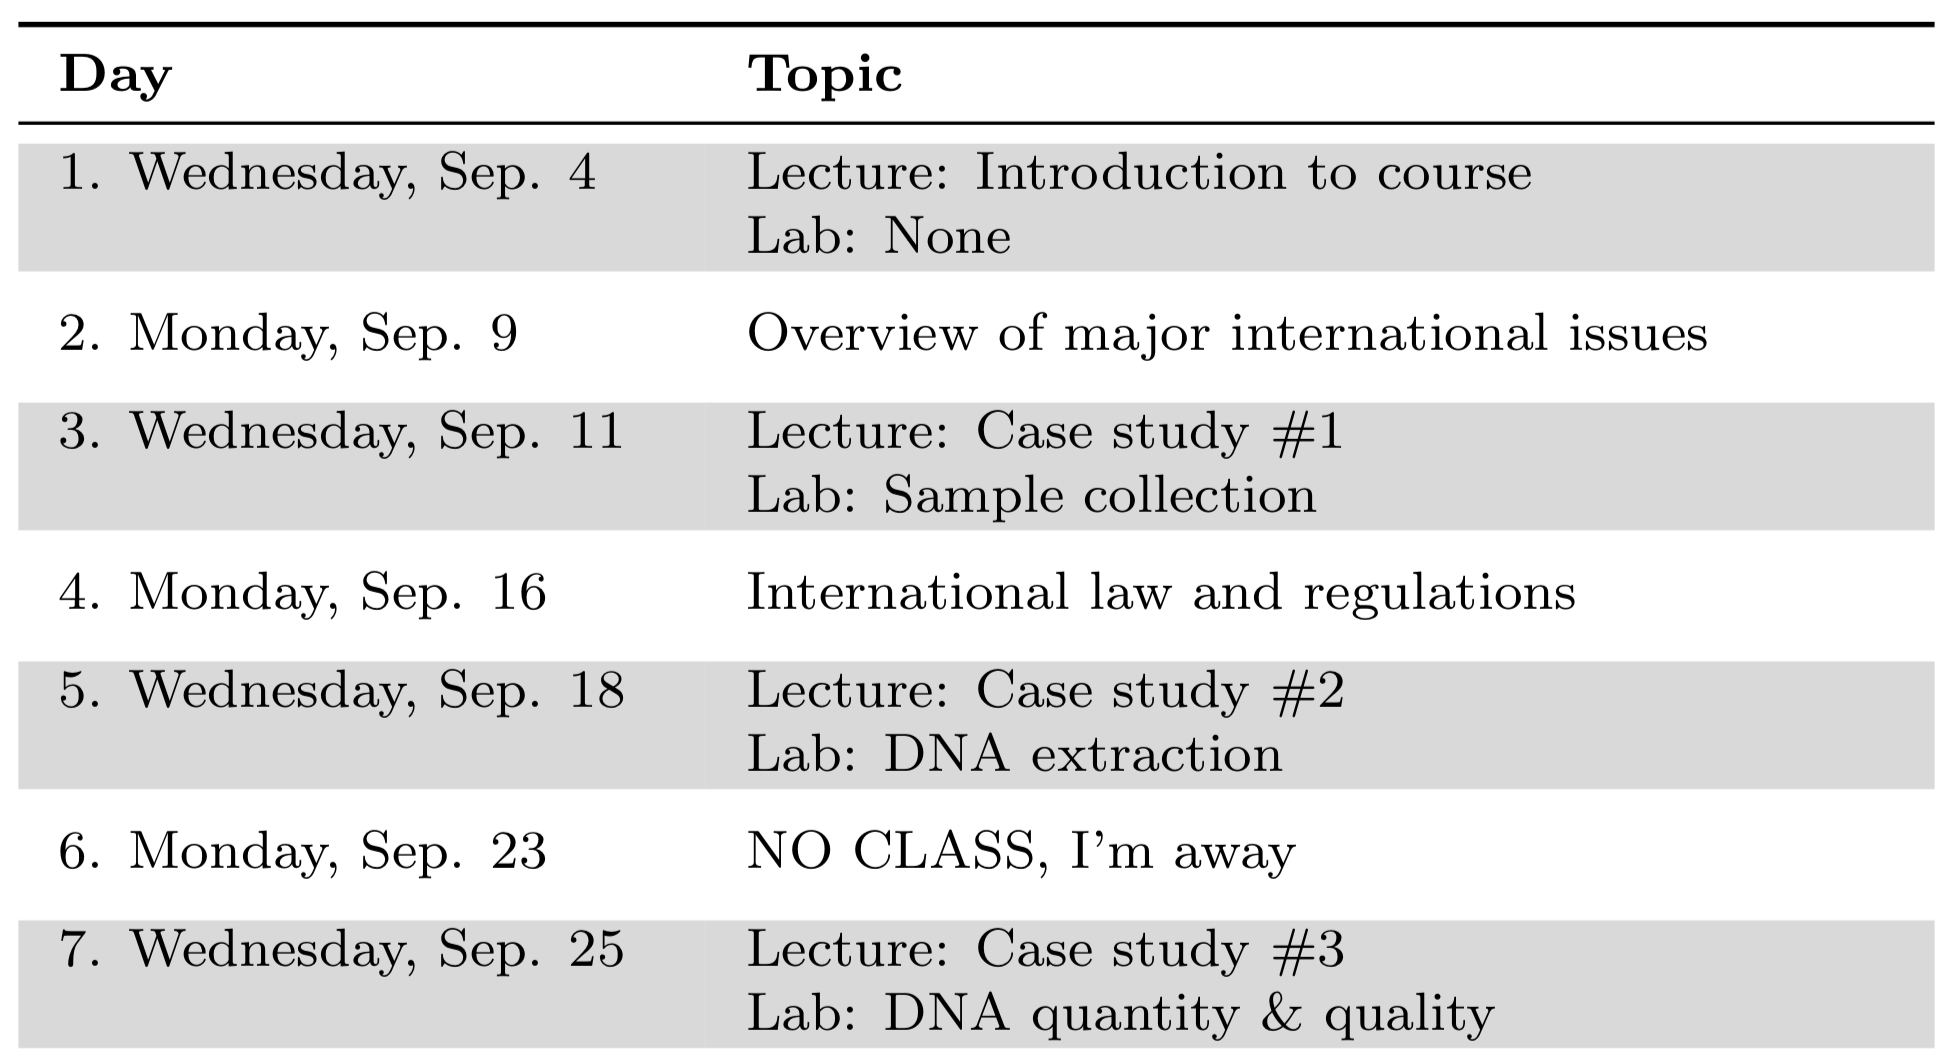
\includegraphics[width=0.7\textwidth]{figures/schedule.png}
	\end{center}
\end{frame}


%-------------------------%
%  Case Studies I         %
%-------------------------%
\begin{frame}[t]
\frametitle{Case Studies}
\framesubtitle{Structure}
\vspace{0.5cm}

	\begin{enumerate}
		\item Pick a case study---I have preliminary readings
		\medskip
		\item Conduct in-depth research:
			\begin{itemize}
				\item What are the main drivers?
				\item What are the implications for the species/people/environments involved?
				\item What are the major legal issues?
				\item Who is/should be responsible for enforcing them?
			\end{itemize}
		\medskip
		\item Teach the class about this case study
			\begin{itemize}
				\item Presentation, discussion, and/or activity (\textcolor{myblue}{can't just be a presentation})
				\item Should have some \textcolor{myblue}{required reading} for the class!
			\end{itemize}	
	\end{enumerate}
\end{frame}


%-------------------------%
%  Case Studies II        %
%-------------------------%
\begin{frame}[t]
\frametitle{Case Studies}
\vspace{0.5cm}

	Will work in teams of 2--3\\
	\vspace{0.5cm}
	Will have full class time for this\\
	\vspace{0.5cm}

	\begin{center}
		\begin{tabular}{p{6cm} r}
			\toprule
			\textbf{Component} & \textbf{\% of grade}\\
			\addlinespace
			\midrule
			Thoroughness of research & 40\%\\
			\addlinespace
			Clarity and effectiveness of presentation/discussion/activity & 40\%\\
			\addlinespace
			Peer evaluations & 20\%\\
			\midrule
			\textbf{Total} & \textbf{100\%}\\
			\bottomrule
		\end{tabular}
	\end{center}
\end{frame}


%-------------------------%
%  Lab                    %
%-------------------------%
\begin{frame}[t]
\frametitle{Lab}
\vspace{0.5cm}

	\textbf{Goal:}\\
	Learn the theory and techniques associated with molecular species identification\\
	
	\vspace{1.0cm}
	
	Apply this to food purchased at local restaurants
\end{frame}


%-------------------------%
%  Lab II                 %
%-------------------------%
\begin{frame}[t]

	\begin{tikzpicture}[overlay]
		\node at (5.5, -1.0) (node1) {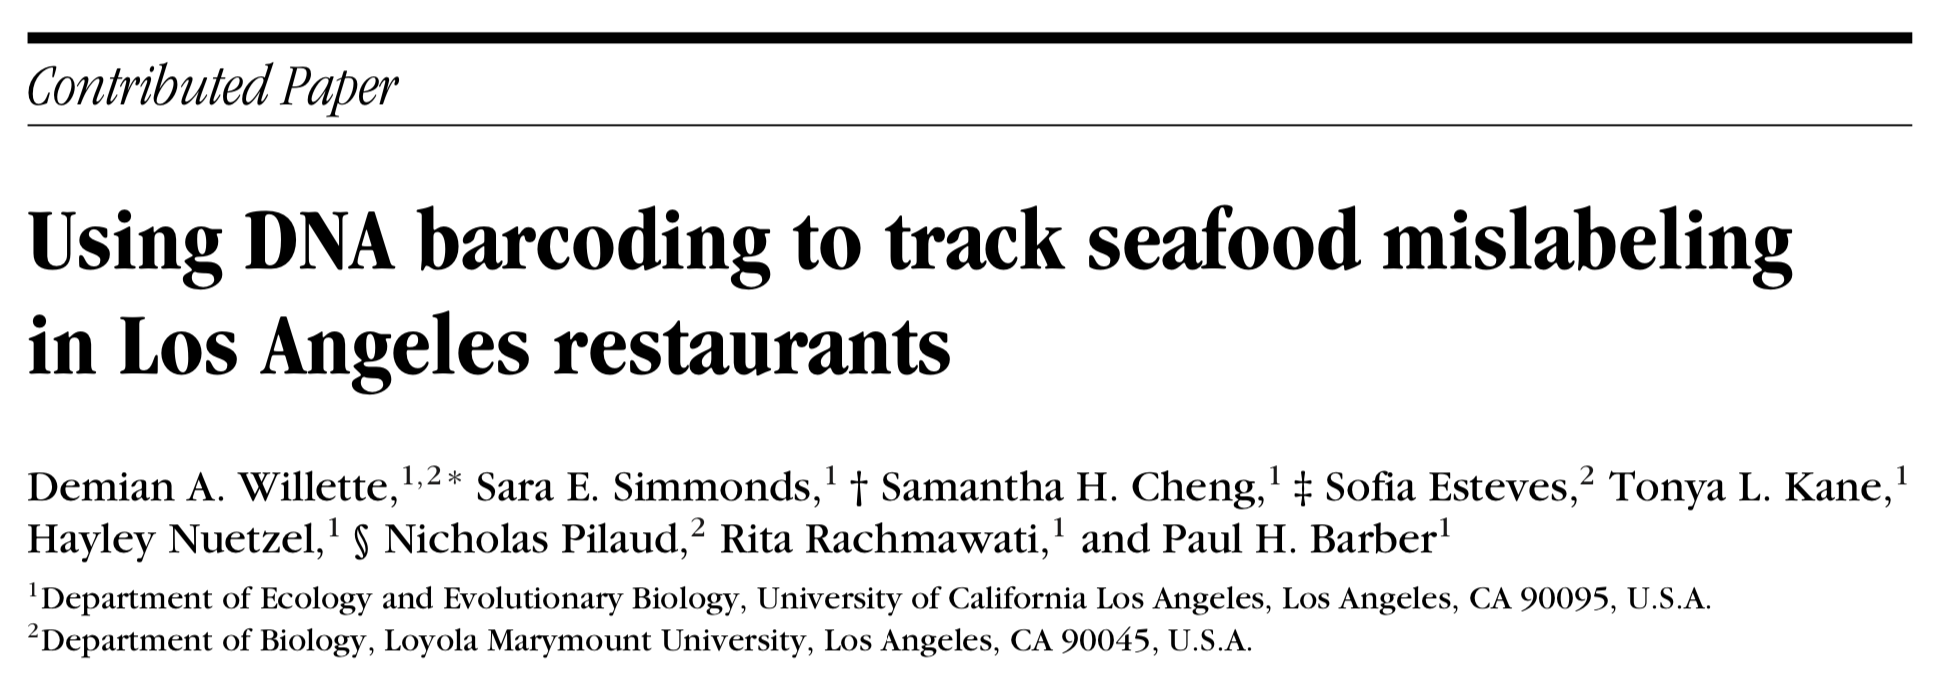
\includegraphics[width=0.7\textwidth]{figures/mislabeled1.png}};
		\node at (1.5, -5.5) (node1) {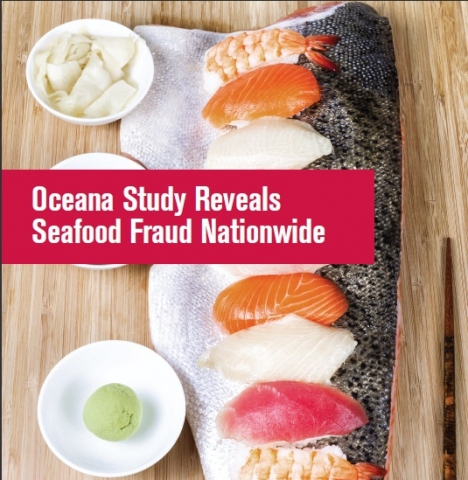
\includegraphics[width=0.35\textwidth]{figures/mislabeled3.jpg}};
		\node at (8.0, -5.5) (node1) {
\includegraphics[width=0.7\textwidth]{figures/mislabeled2.png}};
	\end{tikzpicture}
\end{frame}


%-------------------------%
%  Case study assignment  %
%-------------------------%
\begin{frame}[t]
\frametitle{Case Study Assignment}
\vspace{0.5cm}

	\begin{columns}
		\begin{column}{0.5\textwidth}
			\textcolor{myblue}{Case Study \#1: Sep. 11, Elephant ivory}\\
			\bigskip
			\textcolor{myblue}{Case Study \#2: Sep. 18, Rhino horn}\\
			\bigskip
			Case Study \#3: Sep. 25, Pangolins\\
			\bigskip
			Case Study \#4: Oct. 2, Bear bile\\
			\bigskip
			Case Study \#5: Oct. 9, Caviar\\
		\end{column}
		
		\begin{column}{0.5\textwidth}
			Case Study \#6: Oct. 16, Timber\\
			\bigskip
			Case Study \#7: Oct. 30, Shark fins\\
			\bigskip
			Case Study \#8: Nov. 6, Tigers\\
			\bigskip
			Case Study \#9: Nov. 20, Plant/herbal ingredients\\
			\bigskip
			Case Study \#10: Nov. 27, Birds\\
		\end{column}
	\end{columns}	
\end{frame}

	
\end{document}